\chapter{Solução}
\label{cha:solucao}

\section{Arquitetura}
\label{sec:arquitetura}
A arquitetura usada para este projeto foi a arquitetura sugerida no enunciado denominada de \textit{N Version Programming}.

\begin{figure}[htpb]
  \centering
  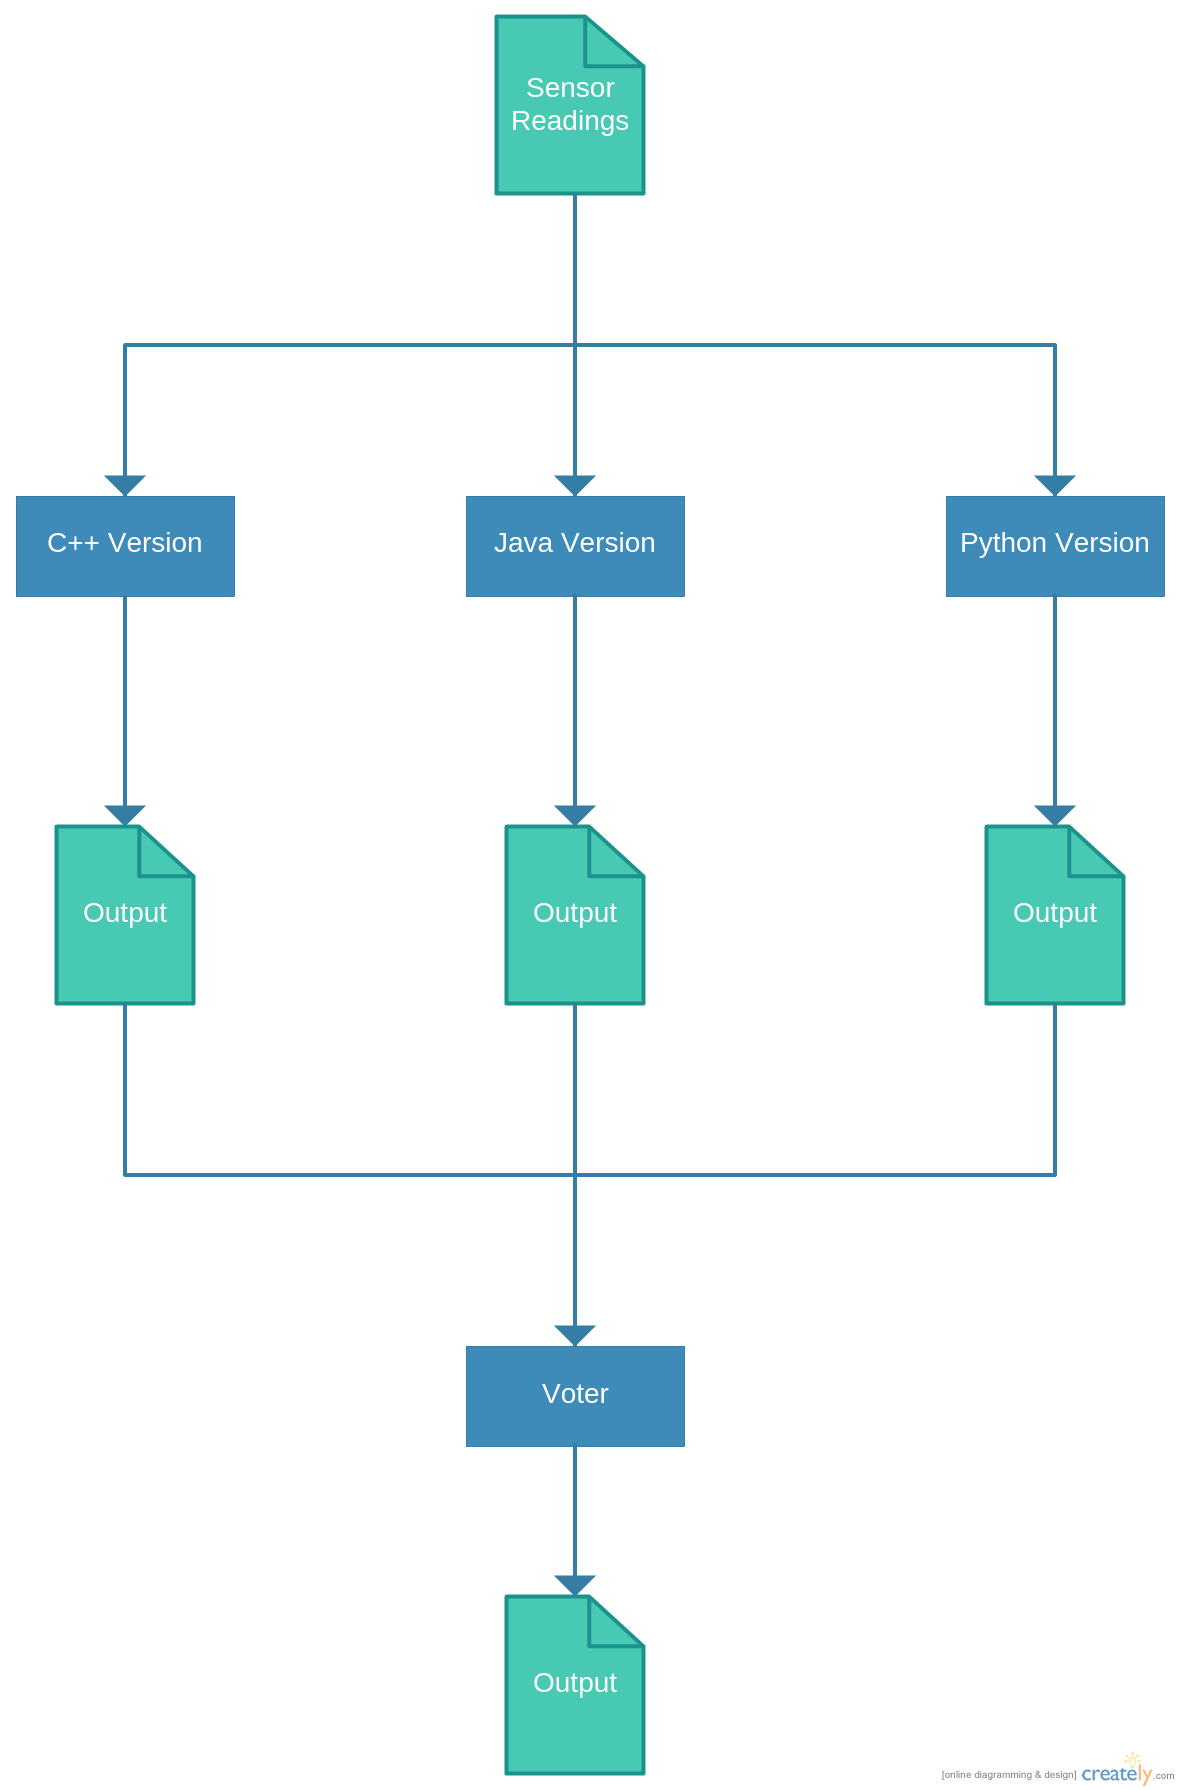
\includegraphics[scale=0.15]{arquitecture.png}
  \caption{Arquitetura}
  \label{fig:arquitecture}
\end{figure}

Como demonstra a figura~\ref{fig:arquitecture} existem três versões de implementação da lógica de cálculo da dosagem de insulina a ser
administrada ao paciente. Estas implementações vão ler um ficheiro de texto com as leituras da glucose no sangue
provenientes dos sensores, calcular as dosagens a injetar a cada três minutos e escrever essas dosagens num ficheiro de
texto.\par
Tendo os três ficheiros com os resultados das dosagens calculadas por cada versão, foi implementado um votador que lê
os três ficheiros e escreve para um ficheiro de saída o valor combinado das três versões.

\section{Diversidade}
\label{sec:diversidade}
Para garantir a diversidade e a unicidade de cada versão, cada uma delas foi distribuida por um dos elementos do grupo.
Cada elemento escolheu uma linguagem para implementar a sua versão, as restrições e validações aplicadas ao ficheiro de
leituras sem que houvesse qualquer tipo de partilha de informação entre os membros do grupo nesta fase da conceção, à 
excepção do formato do ficheiro com as dosagens a serem administradas ao paciente.\par
Depois de implementadas as três versões, os membros do grupo juntaram-se para desenvolver o votador.\par
As linguagens usadas para implementar as versões foram: \textit{C++, Java, Python} e o votador foi desenvolvido em
\textit{Python}
